\problemname{Sifferkryptot}
Alice har hittat på ett revolutionärt chiffer som ingen kommer kunna lösa!
Så här går det till: man tar strängen som ska krypteras, och byter ut varje bokstav mot deras position i alfabetet (A blir $1$, B blir $2$, $C$ blir 3 o.s.v upp till Ö som blir $29$).
När hon gjort detta upptäcker hon det stora problemet med chiffret: det går inte alltid att avkoda entydigt! 

\begin{figure}[h]
  \centering
  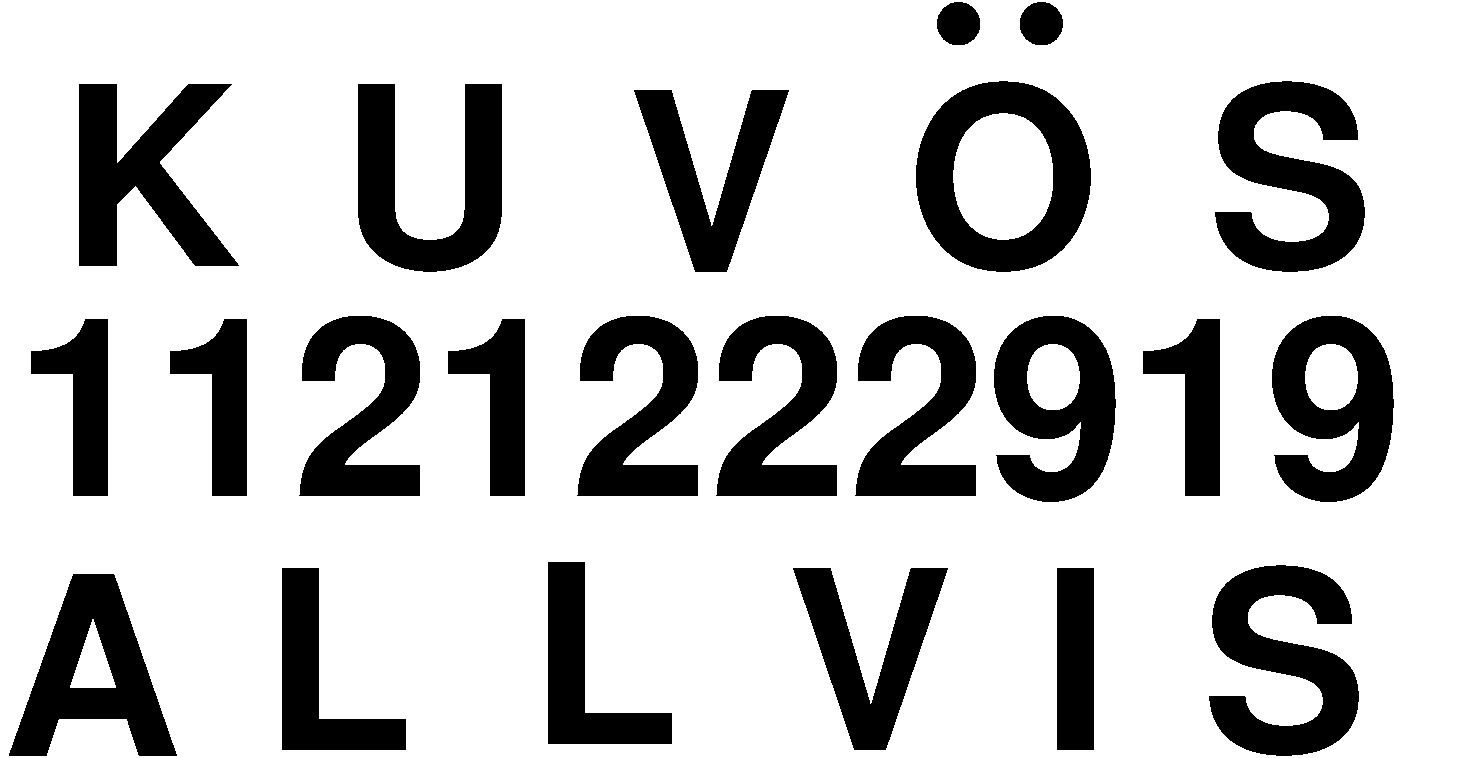
\includegraphics[width=0.6\textwidth]{sifferkrypto.pdf}
  \caption{Exempel på missuppfattning som kan ske med Alice nya krypto.}
\end{figure}

Skriv ett program som läser in ett krypterat meddelande och skriver ut hur många olika ursprungssträngar som skulle kunna ha gett upphov till detta meddelande.
För givna indata finns alltid minst en möjlig ursprungssträng.

\section*{Indata}
Indatan består av en enda rad med minst $1$ och högst $15$ siffror.

\section*{Utdata}
Skriv ut ett enda heltal: antalet ursprungssträngar som skulle kunna gett upphov till det krypterade meddelandet.

\section*{Poängsättning}
Din lösning kommer att testas på en mängd testfallsgrupper.
För att få poäng för en grupp så måste du klara alla testfall i gruppen.

\noindent
\begin{tabular}{| l | l | p{12cm} |}
  \hline
  \textbf{Grupp} & \textbf{Poäng} & \textbf{Gränser} \\ \hline
  $1$    & $40$      & För varje tre på varandra följande siffror är minst en av dessa varken $1$ eller $2$. \\ \hline
  $2$    & $60$      & Inga ytterligare begränsningar. \\ \hline
\end{tabular}

\section*{Förklaring av exempelfall}
I det första exempelfallet är de sex möjliga ursprungssträngarna CBCABDJ, CWLDJ, CWAXJ, CWABDJ, CBCAXJ, och CBCLDJ.
